\begin{figure}[t]
  \centering
  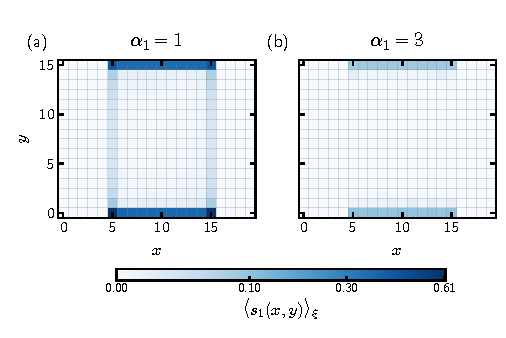
\includegraphics[width=\columnwidth]{entropy_contours_hard_n20x32_alpha1_1_3.pdf}
  \caption{\textbf{Entanglement contours at matched size.}
  Von Neumann entanglement contours for (a) $\alpha_1=1$ and
  (b) $\alpha_1=3$, with $N_x=20$, $N_y=32$, $\alpha_2=30$, and
  hard walls. Each panel shows the cellwise average over $100$ independent
  pure-state trajectories after $64=2N_y$ cycles of perfect-correction
  dynamics, using $n_{\mathrm{shell}}=1$ and raster-$y$ ordering.
  The initial random half-filled pure state undergoes the hard-wall exterior
  preparation. The fixed subsystem is $[0,20)\times[0,16)$; each pixel sums
  both orbitals. Contours are computed separately before trajectory averaging,
  with no average over subsystem origins. Both panels share the same
  square-root-normalized Blues scale; gray lines mark unit cells.}
  \label{fig:entropy-contour-alpha-comparison}
\end{figure}
